\documentclass[journal]{vgtc}                     % final (journal style)
%\documentclass[journal,hideappendix]{vgtc}        % final (journal style) without appendices
%\documentclass[review,journal]{vgtc}              % review (journal style)
%\documentclass[review,journal,hideappendix]{vgtc} % review (journal style)
%\documentclass[widereview]{vgtc}                  % wide-spaced review
%\documentclass[preprint,journal]{vgtc}            % preprint (journal style)
\usepackage[demo]{graphicx}
\usepackage{adjustbox}


%% Uncomment one of the lines above depending on where your paper is
%% in the conference process. ``review'' and ``widereview'' are for review
%% submission, ``preprint'' is for pre-publication in an open access repository,
%% and the final version doesn't use a specific qualifier.

%% If you are submitting a paper to a conference for review with a double
%% blind reviewing process, please use one of the ``review'' options and replace the value ``0'' below with your
%% OnlineID. Otherwise, you may safely leave it at ``0''.
\onlineid{0}

%% In preprint mode you may define your own headline. If not, the default IEEE copyright message will appear in preprint mode.
%\preprinttext{To appear in IEEE Transactions on Visualization and Computer Graphics.}

%% In preprint mode, this adds a link to the version of the paper on IEEEXplore
%% Uncomment this line when you produce a preprint version of the article 
%% after the article receives a DOI for the paper from IEEE
%\ieeedoi{xx.xxxx/TVCG.201x.xxxxxxx}

%% declare the category of your paper, only shown in review mode
\vgtccategory{Research}

%% please declare the paper type of your paper to help reviewers, only shown in review mode
%% choices:
%% * algorithm/technique
%% * application/design study
%% * evaluation
%% * system
%% * theory/model
%% Paper title.
\title{CitiBike Usage Visualization}

%% Author ORCID IDs should be specified using \authororcid like below inside
%% of the \author command. ORCID IDs can be registered at https://orcid.org/.
%% Include only the 16-digit dashed ID.
\author{%
  \textit{Narendra Sairam Murthy Buddhavarapu,
  Aryaman Rao Nagineni}
}

\authorfooter{
  %% insert punctuation at end of each item
  \item
  	Narendra Sairam Murthy Buddhavarapu is with University of Illinois at Chicago.
  	E-mail: nbuddh2@uic.edu
  \item
  	Aryaman Rao Nagineni is with University of Illinois at Chicago.
  	E-mail: anagin2@uic.edu
}



%% Keywords that describe your work. Will show as 'Index Terms' in journal
%% please capitalize first letter and insert punctuation after last keyword
%% A teaser figure can be included as follows

%% Uncomment below to disable the manuscript note
\renewcommand{\manuscriptnotetxt}{}

%% Copyright space is enabled by default as required by guidelines.
%% It is disabled by the 'review' option or via the following command:
%\nocopyrightspace


%%%%%%%%%%%%%%%%%%%%%%%%%%%%%%%%%%%%%%%%%%%%%%%%%%%%%%%%%%%%%%%%
%%%%%%%%%%%%%%%%%%%%%% LOAD PACKAGES %%%%%%%%%%%%%%%%%%%%%%%%%%%
%%%%%%%%%%%%%%%%%%%%%%%%%%%%%%%%%%%%%%%%%%%%%%%%%%%%%%%%%%%%%%%%

%% Tell graphicx where to find files for figures when calling \includegraphics.
%% Note that due to the \DeclareGraphicsExtensions{} call it is no longer necessary
%% to provide the the path and extension of a graphics file:
%% \includegraphics{diamondrule} is completely sufficient.
\graphicspath{{figs/}{figures/}{pictures/}{images/}{./}} % where to search for the images

%% Only used in the template examples. You can remove these lines.
\usepackage{tabu}                      % only used for the table example
\usepackage{booktabs}                  % only used for the table example
\usepackage{lipsum}                    % used to generate placeholder text
\usepackage{mwe}                       % used to generate placeholder figures

%% We encourage the use of mathptmx for consistent usage of times font
%% throughout the proceedings. However, if you encounter conflicts
%% with other math-related packages, you may want to disable it.
\usepackage{mathptmx}                  % use matching math font
\usepackage{indentfirst} 
\begin{document}

%%%%%%%%%%%%%%%%%%%%%%%%%%%%%%%%%%%%%%%%%%%%%%%%%%%%%%%%%%%%%%%%
%%%%%%%%%%%%%%%%%%%%%% START OF THE PAPER %%%%%%%%%%%%%%%%%%%%%%
%%%%%%%%%%%%%%%%%%%%%%%%%%%%%%%%%%%%%%%%%%%%%%%%%%%%%%%%%%%%%%%%

%% The ``\maketitle'' command must be the first command after the
%% ``\begin{document}'' command. It prepares and prints the title block.
%% the only exception to this rule is the \firstsection command
\maketitle

\firstsection{Abstract}
 \textit{\textbf{ Abstract: The popularity of bike sharing programs has skyrocketed in recent years, with more and more cities across the globe introducing these programs to provide an alternative to traditional transportation modes. Citi Bike, a bike sharing program in New York City, is one of the most extensive bike sharing programs in the world, with over 300 stations and 14,000 bikes distributed throughout Manhattan, Brooklyn, Queens, and Jersey City.
Despite the wide availability of Citi Bike stations, users have reported difficulties in finding available bikes or empty docks to return their bikes. This issue can be frustrating for riders, especially when they are in a hurry to reach their destination or have limited time to explore the city. Therefore, it is essential to understand the factors that contribute to the demand and usage of Citi Bike and its stations.}} \href{https://github.com/nbuddh2/Citi-Bike-Vis}{https://github.com/nbuddh2/Citi-Bike-Vis}

\section{Introduction}




%% \section{Introduction} %for journal use above \firstsection{..} instead
In recent years, bike-sharing programs have emerged as a promising solution to the transportation and environmental challenges faced by urban areas around the world. Bikes are an important part of public transportation since they are environment-friendly, cheap and easy to adapt to different environments. They also provide a popular form of recreation. Nowadays, with the emphasis on healthy living style, bikes become even more popular. The bike-sharing systems provide people an opportunity to use bicycles anytime and anywhere without the limitation of inconvenience \cite{Parkes et al.}. People initially tried and failed to introduce bike-sharing schemes in the 1960s due to the technical limitations such as tracking bikes and instant payment. However, nowadays, technological advances, such as bike tracking, solar powered sensors, mobile phones and wide-area internet and online aces, have helped transform bike-sharing from an aspiration to reality. \cite{lamport94}

The Citi Bike program in New York City has been a standout example of the success of such programs, offering an affordable, eco-friendly, and convenient means of transportation. With over 10,000 bikes and 700 stations, the program has become an essential part of the city's transportation landscape. Despite the wide availability of Citi Bike stations, users have reported difficulties in finding available bikes or empty docks to return their bikes.\cite{Faghih-imani} This issue can be frustrating for riders, especially when they are in a hurry to reach their destination or have limited time to explore the city. Therefore, it is essential to understand the factors that contribute to the demand and usage of Citi Bike and its stations. The program has been growing in popularity over the years, and as a result, the demand for bicycles has increased. To meet this demand, the City Bike program has expanded by adding more bicycles and docking stations throughout the city. However, despite the expansion of the program, there have been several issues that have arisen, including the uneven distribution of bicycles throughout the city, the lack of available bicycles at popular docking stations, and the inability of users to visualize the usage of bicycles in real-time. These issues have led to frustration among users and have the potential to negatively impact the overall success of the program.\cite{Goodman A} This paper will explore the problem of the uneven distribution of bicycles in New York City and propose a solution in the form of a visualization tool.

 As potential users of Citi Bike, we were motivated to investigate this issue further. During our visit to New York City, we experienced firsthand the challenges of accessing bikes and empty docks, even with four stations located within two blocks of our hotel \cite{M}. We were surprised by the limited availability of bikes despite the widespread distribution of stations throughout the city.We hypothesized that several factors could influence the demand and usage of Citi Bike stations, such as nearby infrastructure, weather, seasons, users' demographic profile, and borrowing and returning hours. We wanted to explore the impact of these factors on the demand for bikes, the number of available docks, and the user experience.

 
The problem with the Citi Bike program in New York City is the less supply of bicycles where there is high demand throughout the city. The current distribution of bicycles is not optimal and does not adequately address the needs of all users. There are certain areas of the city where there are not enough bicycles, while in other areas, there are too many. This problem is important because it affects the overall success of the Citi Bike program \cite{Meng}. If users are unable to rent or return bicycles, they may become frustrated and opt for other modes of transportation. This could result in a decrease in the use of the Citi Bikes, which would have negative environmental and economic impacts. To ensure the success of such ventures, it is useful to study the operation of existing public bicycle programs to identify features that improve the effectiveness of bike share scheme implementations. For instance, a comparison of bike share schemes in China revealed that government-led investment, enforced bicycle lanes and technologically sophisticated equipment greatly boosted the performance of bike share schemes\cite{Zhao J}. Making public bicycles available to non registered users can increase the number of trips taken and introduce new flow patterns between docking stations compared to a system reserved for use by subscribers only.

\parbox{\linewidth}{
        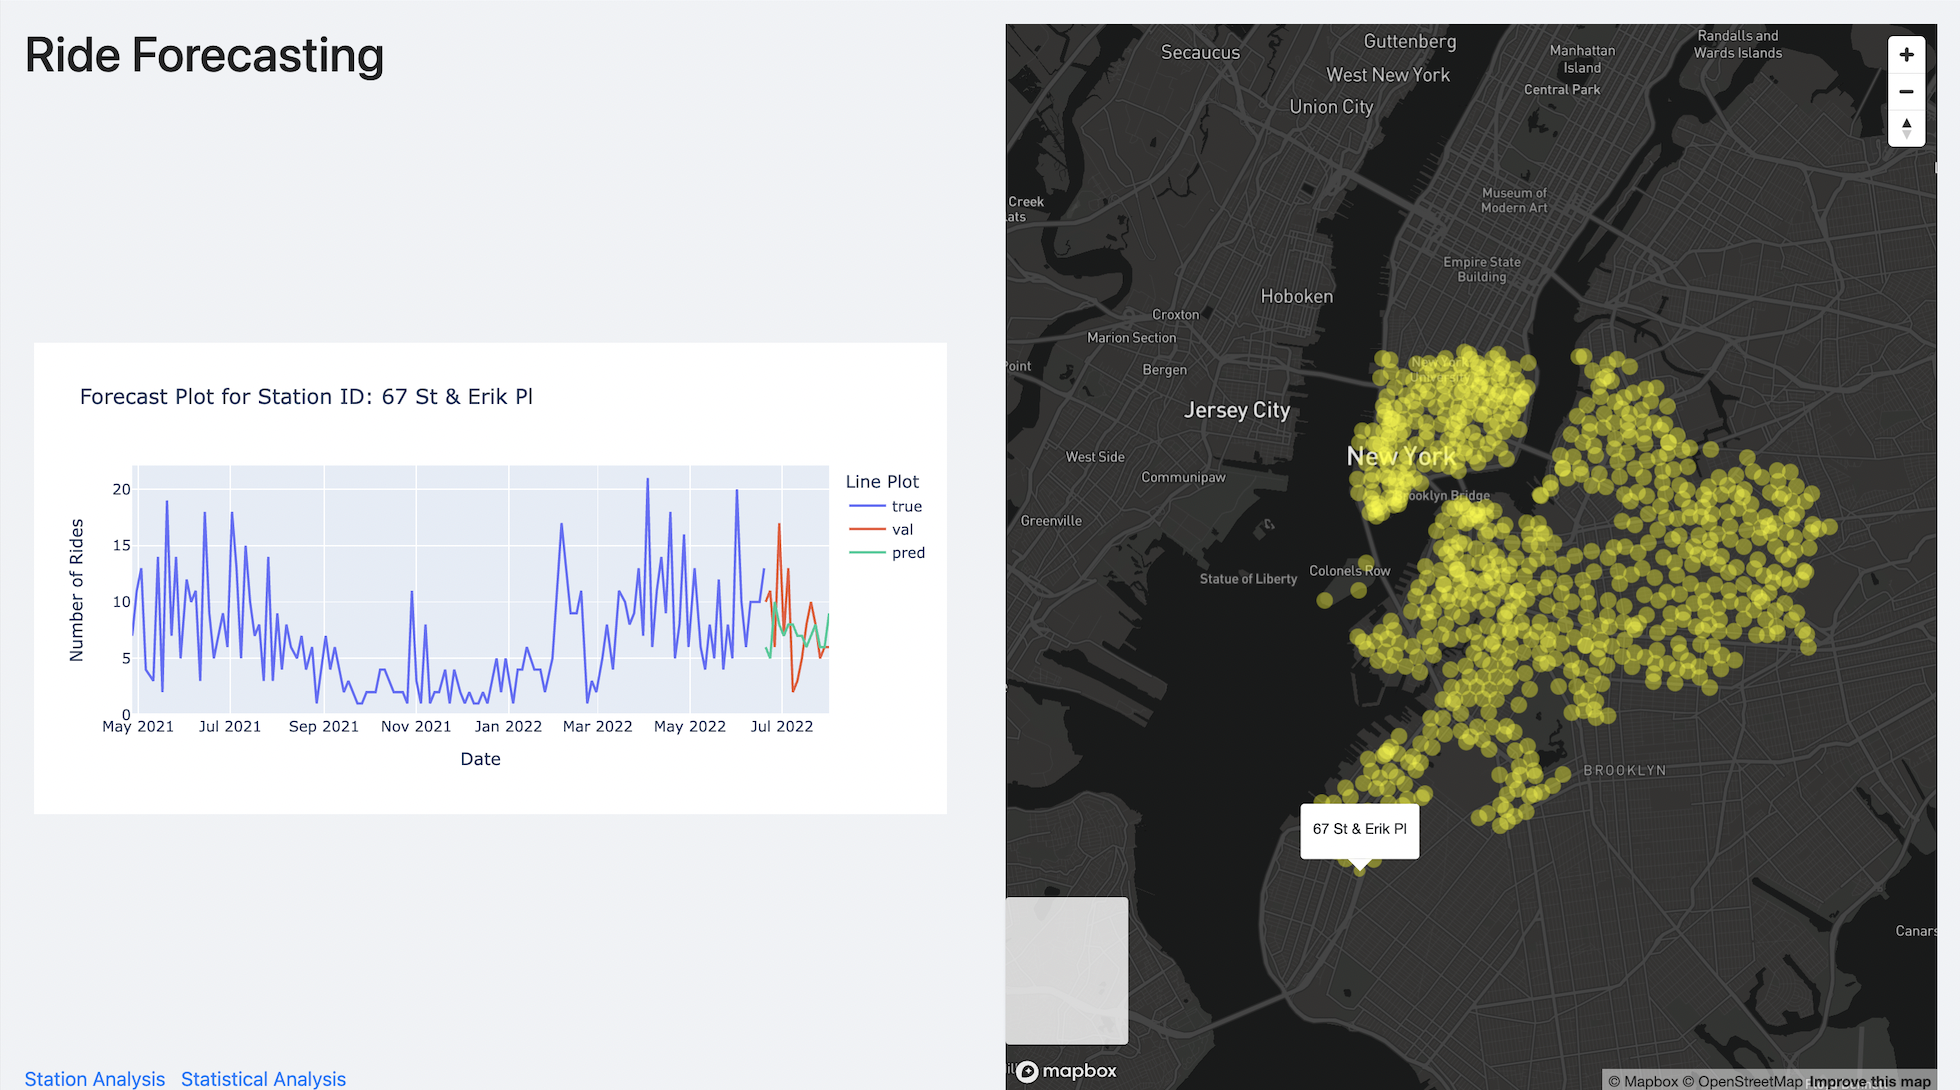
\includegraphics[width=3.4in, height=2in]{figs/ride.png}\\
        \captionof{figure}{Ride forecasting of a station selected on the map }}
        
To address this problem, we developed a visualization tool that will allow users to visualize the usage and analytics of bicycles in real-time. The tool will provide users with information on the usage of the citi bike bicycles and analysis which provides a visual representation of the analysis, statistics and future inference of Citi Bike stations across the city. This information is helpful in understanding the demand for Citi Bikes in different areas of the city and can be used to optimize the distribution of stations. This will enable users to plan their trips more efficiently and avoid areas where there are no available bicycles or docking stations and will also help the company's policy/decision makers to plan accordingly and enhance their ecosystem.


\section{Related work}
\textbf{Understanding the Usage of Public Bicycle-Sharing Systems} by Chen et al. (2017) \cite{Xiaonan Zhang}: This study analyzed the usage patterns of bike-sharing systems in different cities, including New York City. The authors used data mining techniques to understand the factors affecting the demand for bike-sharing systems.

\textbf{A Comparative Analysis of Bike Sharing Systems in Urban Areas} by Patsakis et al. (2018) \cite{Yuan}: This study compared the bike-sharing systems in different cities, including New York City. The authors analyzed the usage patterns, user satisfaction, and the impact of weather conditions on the usage of the bike-sharing system.

\textbf{Urban Mobility and Equity: A Case Study of Bicycle Sharing in Chicago} by Smith et al. (2018) \cite{August 2020}: This study analyzed the equity issues related to the usage of bike-sharing systems in urban areas. The authors analyzed the socio-economic factors affecting the usage of the bike-sharing system and proposed solutions to address the equity issues.\hfill \break

\parbox{\linewidth}{
        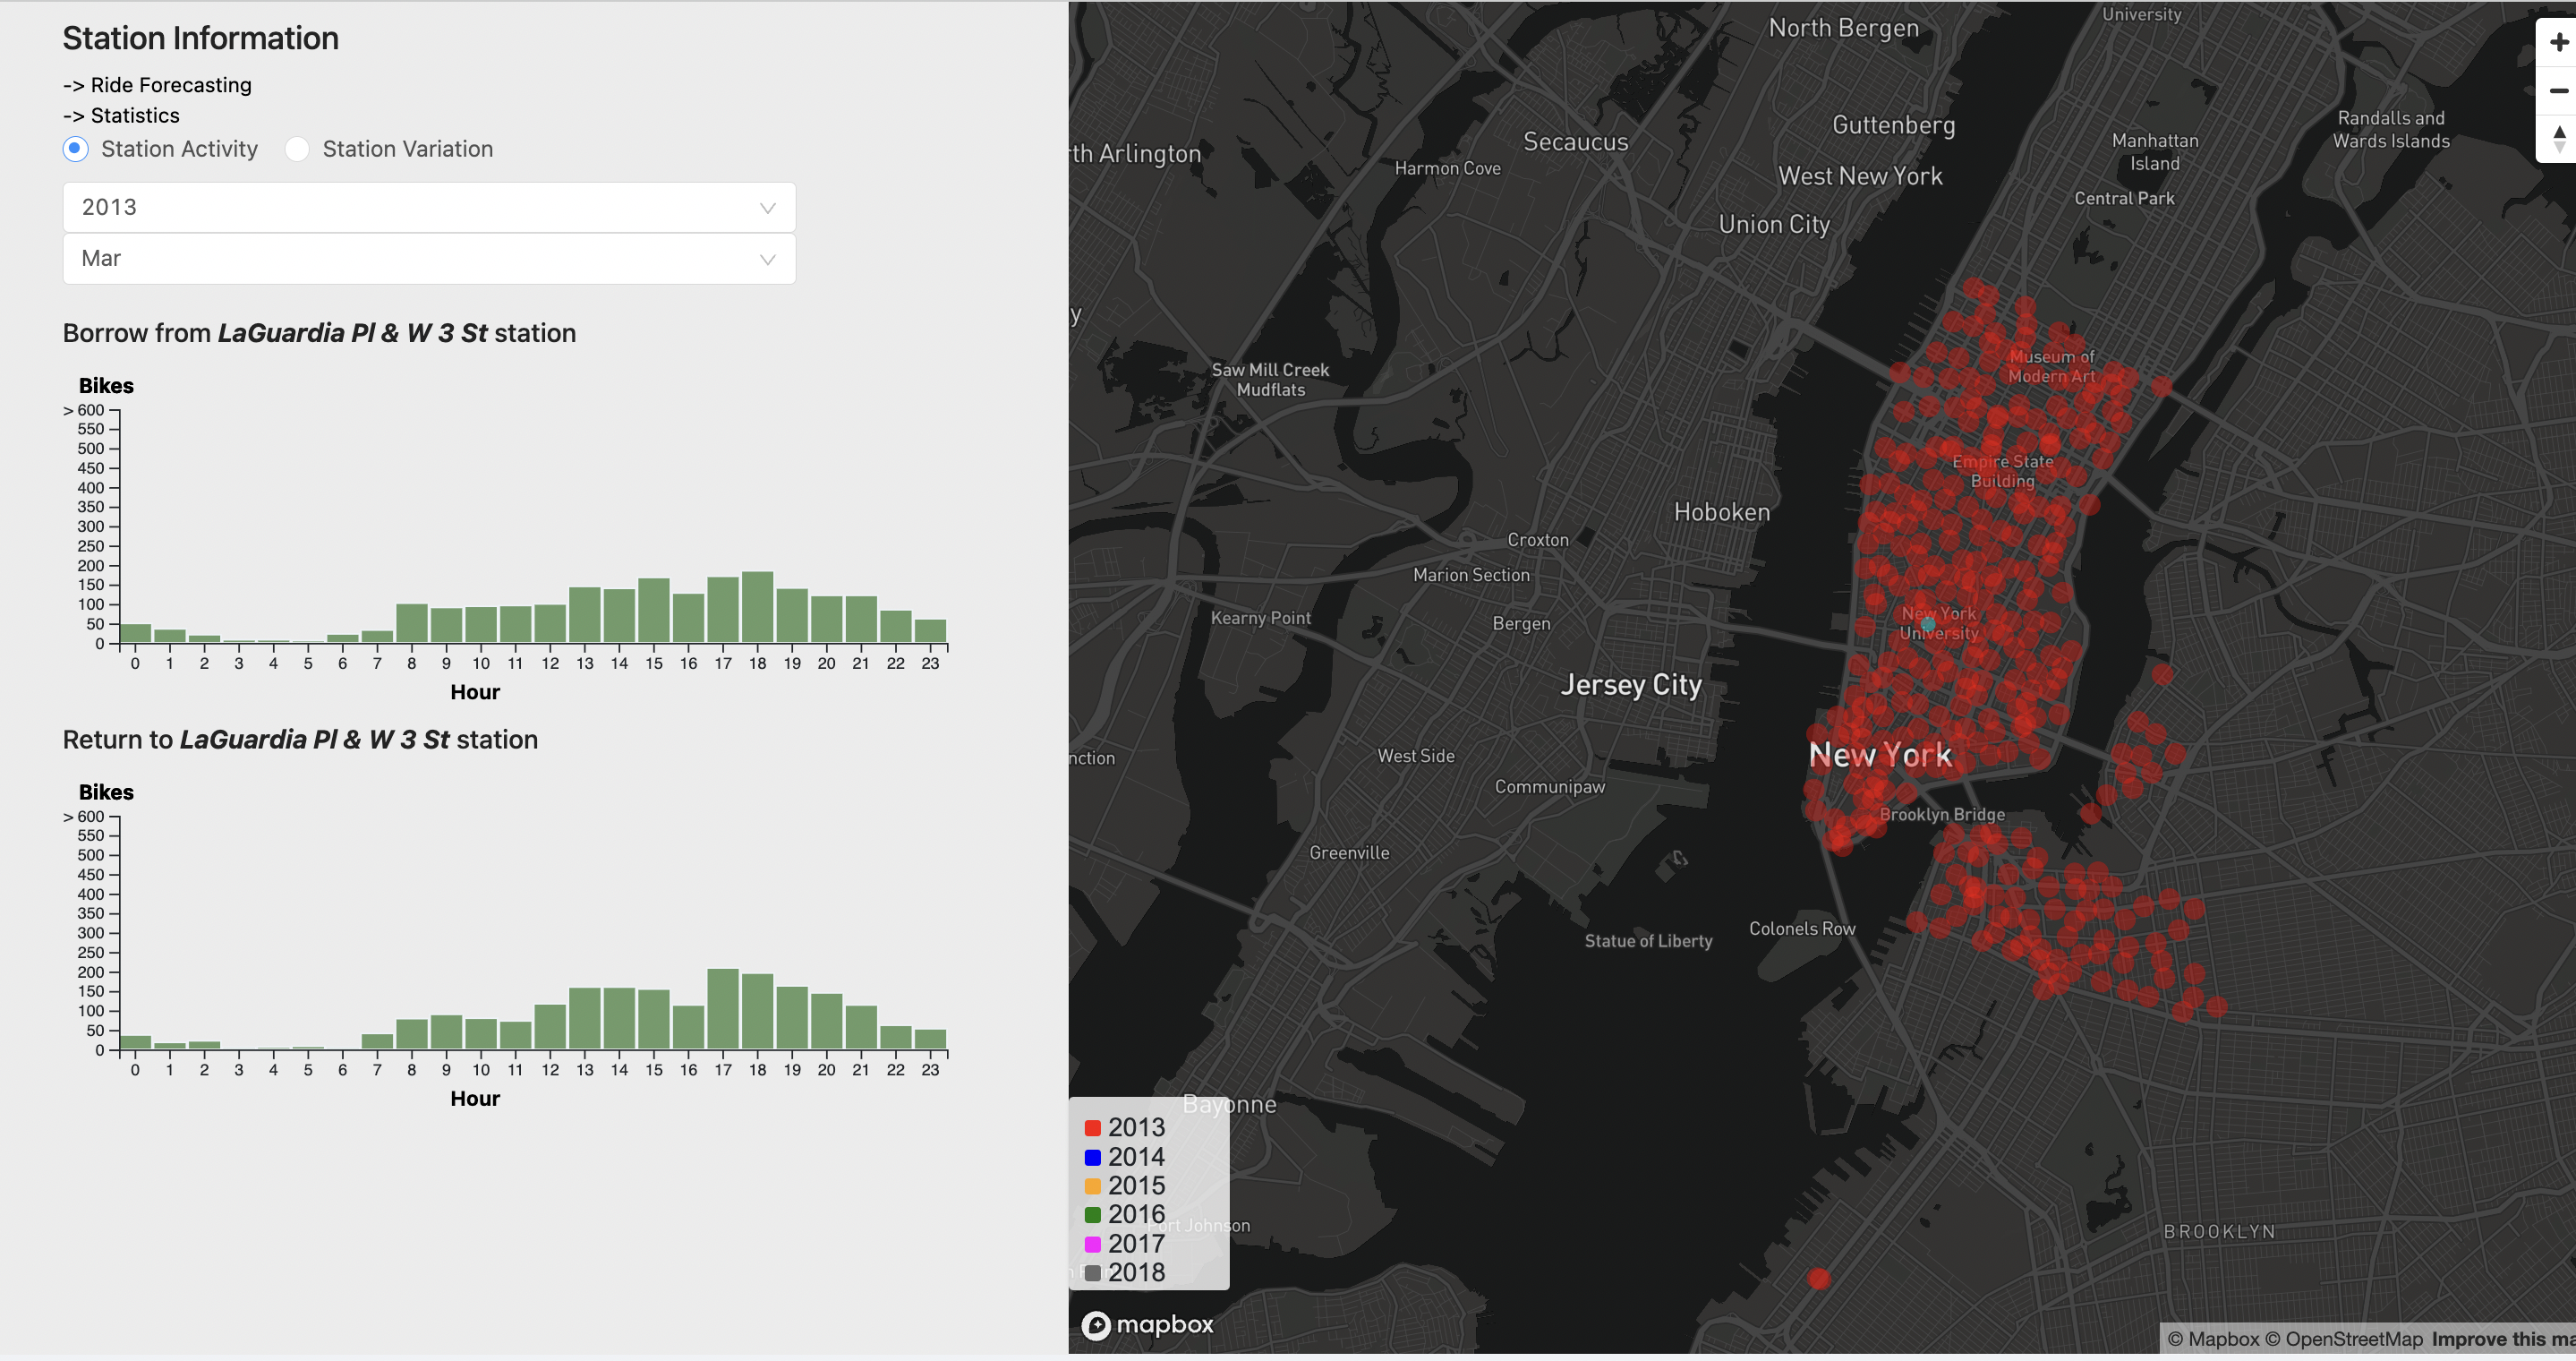
\includegraphics[width=3.3in, height=2in]{figs/analysis.png}\\
        \captionof{figure}{Station Analysis of a station selected }}
        
\textbf{Citi Bike Information Visualization} by Jing Zhang, Tianyang Li, Ziwei Yuan, and Tong Lyu from University of Southern California (2018) \cite{11}. This is a research paper about a visualization project that aims to analyze potential factors that may influence bike-sharing orders through information visualization using Angular, Bootstrap, d3, and Mapbox. The authors used data from Citi Bike Trip Histories and NYC Facilities, among others, to create a map of all stations, accompanied by station information including a summary of borrowed/returned bikes and a summary of annual variation in six years. They also analyzed the infrastructure effect for top 13 popular stations, user age distribution of top six popular stations, and the relationship between precipitation amount and the number of orders.

Our proposed work differs from prior work in several ways. Firstly, the proposed research aims to analyze the usage patterns of the Citi Bike sharing system using data visualization and analytics techniques, whereas prior work used data mining techniques. Secondly, the proposed research includes modules such as Future Forecasting of Each Station, Subscription analysis, Analyzing Top 20 Busy Stations, and Gender Analysis, which were not included in prior work. Furthermore, our proposed work focuses exclusively on the Citi Bike sharing system in New York City, while prior work analyzed bike-sharing systems in different cities. This allows the proposed research to provide a more detailed analysis of the Citi Bike system and provide insights that are specific to New York City. Also our proposed research uses newer technologies such as Deep learning models and big data analytics to analyze the future ride forecasting of the Citi Bike system. Prior work did not utilize these technologies to the same extent.


\section{Data Description}
The dataset used in the paper on Citi Bike Usage Visualization and Analytics in New York City is the Citi Bike trip data, which includes daily trip data over 100 million trip records from 2013 to 2022. The dataset is regularly updated, publicly available, and contains information about the starting and ending points of the trips, the duration of the trips and the demographic information of the users, among other attributes. The dataset also includes geographic information, which allows for the analysis of the distribution of the Citi Bike stations across different neighborhoods in New York City and the spatial patterns of the usage of the Citi Bike sharing system. We pre-processed and cleaned the original data and generated GeoJSON data for the past 10yrs of data. After pre-processing, we found impactful insights such as total number of borrowed bikes per hour of each station for every month, total number of returned bikes per hour of each station for every month of each year. 
While the dataset has several limitations, such as only including trips taken on the Citi Bike sharing system and not including information about the route taken during the trip, it is a valuable resource for analyzing the usage patterns and user behavior of the Citi Bike sharing system in New York City. The large size of the dataset and the richness of the attributes enable the analysis of the temporal and spatial patterns of the usage, the identification of the factors affecting the demand and usage, and the assessment of the equity and sustainability of the system.

\section{Research}
In this paper, we aim to understand the Bike-Share availability in New York city. We analyze over 100 million data entries from 2013 to 2022. We create several maps and plots to visualize the distribution of Bicycles. We provide insights for policy-making and intervention design for future forecasting. Our work differs from related work by covering a longer time period that is every month of ten years of data and a larger geographical scope than most of the other papers, which focus on shorter or specific time periods. One of the main limitations of prior work was the lack of specificity of the analysis to New York City, which was the focus of our paper\cite{YA}. We solved this limitation by obtaining and analyzing the data from the Citi Bike system, which is unique to New York City, providing insights specific to the city. The data was obtained through the Citi Bike system's publicly available data feed, which contained information on each ride, including the start and end station, duration, and user information.
We utilized data visualization and analytics techniques to analyze the data and provide more interactive and accurate insights. This involved using tools such as plotly, d3 for data visualization, Python for data preprocessing, and Deep learning algorithms for demand forecasting. By utilizing these techniques, we were able to create interactive and dynamic visualizations that allowed us to analyze the data more efficiently and effectively.
Our paper also tackled the limitation of prior work in terms of the lack of inclusion of certain modules. For instance, the Future Forecasting of Each Station module was created to predict the demand for each Citi Bike station in the future. We achieved this by analyzing the historical data of each station and training a machine learning algorithm to predict the demand for each station in the future. This module enables city planners to plan for the expansion or reduction of stations as needed, ensuring that the system is optimized for user demand.
\parbox{\linewidth}{
        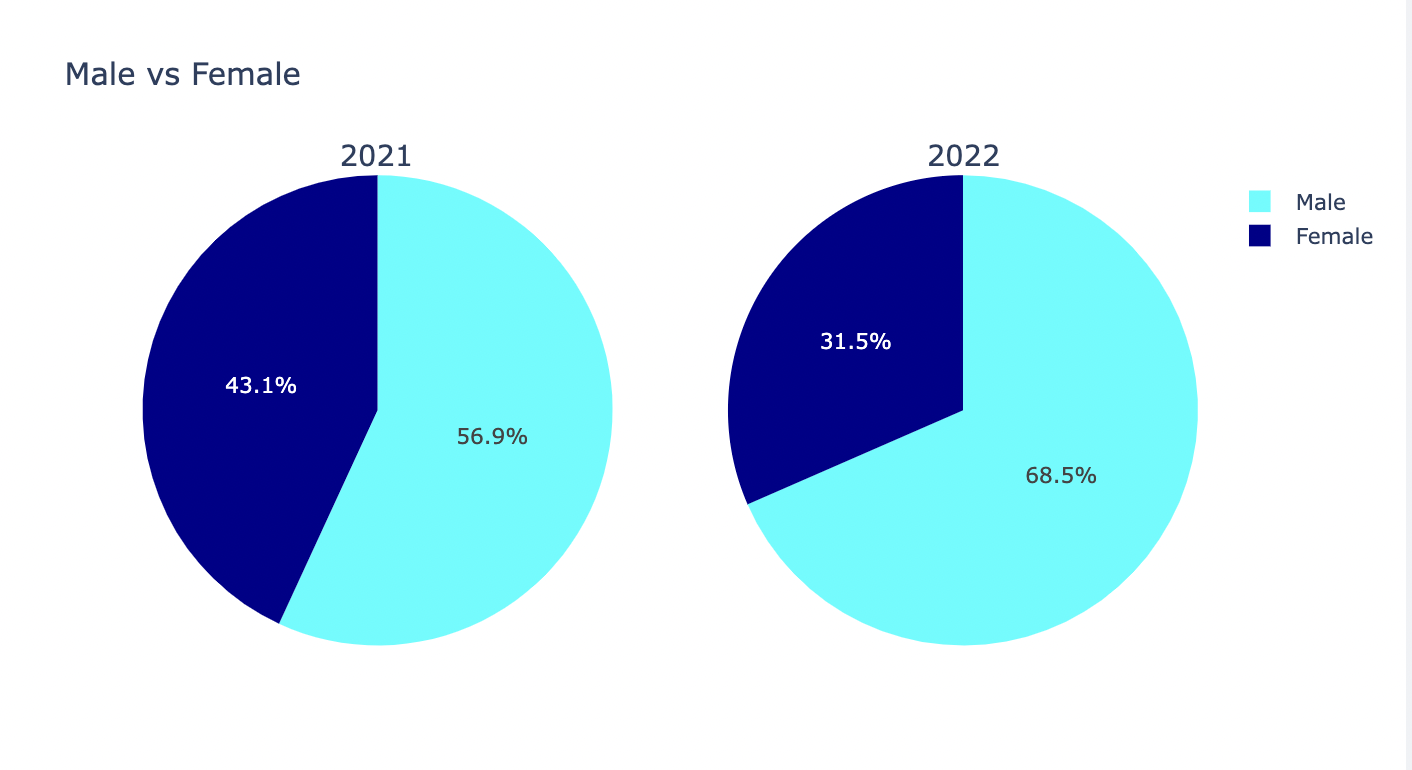
\includegraphics[width=3.31in, height=1.8in]{figs/gender.png}\\
        \captionof{figure}{Gender Analysis of Citi bike usage in years 2021 and 2022}}
Another important module was the Gender Analysis, which provided insights into the gender distribution of the Citi Bike system. We achieved this by analyzing the user data and identifying the gender of each user based on their ride ids. This analysis revealed that the Citi Bike system is used more by male than females, indicating that there is an opportunity for targeted marketing campaigns to increase female ridership.
% In conclusion, our paper tackled several limitations of prior work on bike-sharing systems by utilizing data visualization and analytics techniques, machine learning, big data analytics, and including modules such as Future Forecasting of Each Station and Gender Analysis. Our paper provided more detailed and nuanced insights into the usage patterns of the Citi Bike system, enabling city planners to optimize station locations, bike distribution, and marketing campaigns to increase ridership.

\subsection{Methods}
\begin{enumerate}
\item \textbf{Station Analysis \& Distribution Variation: \cite{11}} This module focuses on analyzing the distribution and availability of the Citi Bikes across New York City. By collecting and processing data on the location and availability of Citi Bike stations, we can gain insights into usage patterns and optimize the distribution of bikes to meet demand.One of the key metrics we analyze is the number of available bikes and docks at each station. By tracking this information over time, we can identify trends and patterns in usage, and make adjustments to ensure that bikes are available when and where they are needed.
\item \textbf{Future Forecasting of Each Station:} In this module, we will use predictive modeling techniques to forecast future demand for each station based on historical usage patterns. This information can be used to optimize the allocation of bikes and ensure that stations are adequately stocked to meet demand.
\item \textbf{Analyzing Top 20 Busy Stations:} This module focuses specifically on the top 20 busiest stations in New York City and explores the factors that contribute to their popularity. We will also examine usage patterns at these stations over time to identify trends and patterns. we can gain insights into usage patterns and identify areas for improvement in the system.
\item \textbf{Demand of Citi Bikes Over the Years:} In this module, we will analyze historical usage patterns to identify trends in demand for Citi Bikes over the years. This information can be used to inform long-term planning and ensure that the program is meeting the changing needs of its users.
\parbox{\linewidth}{
        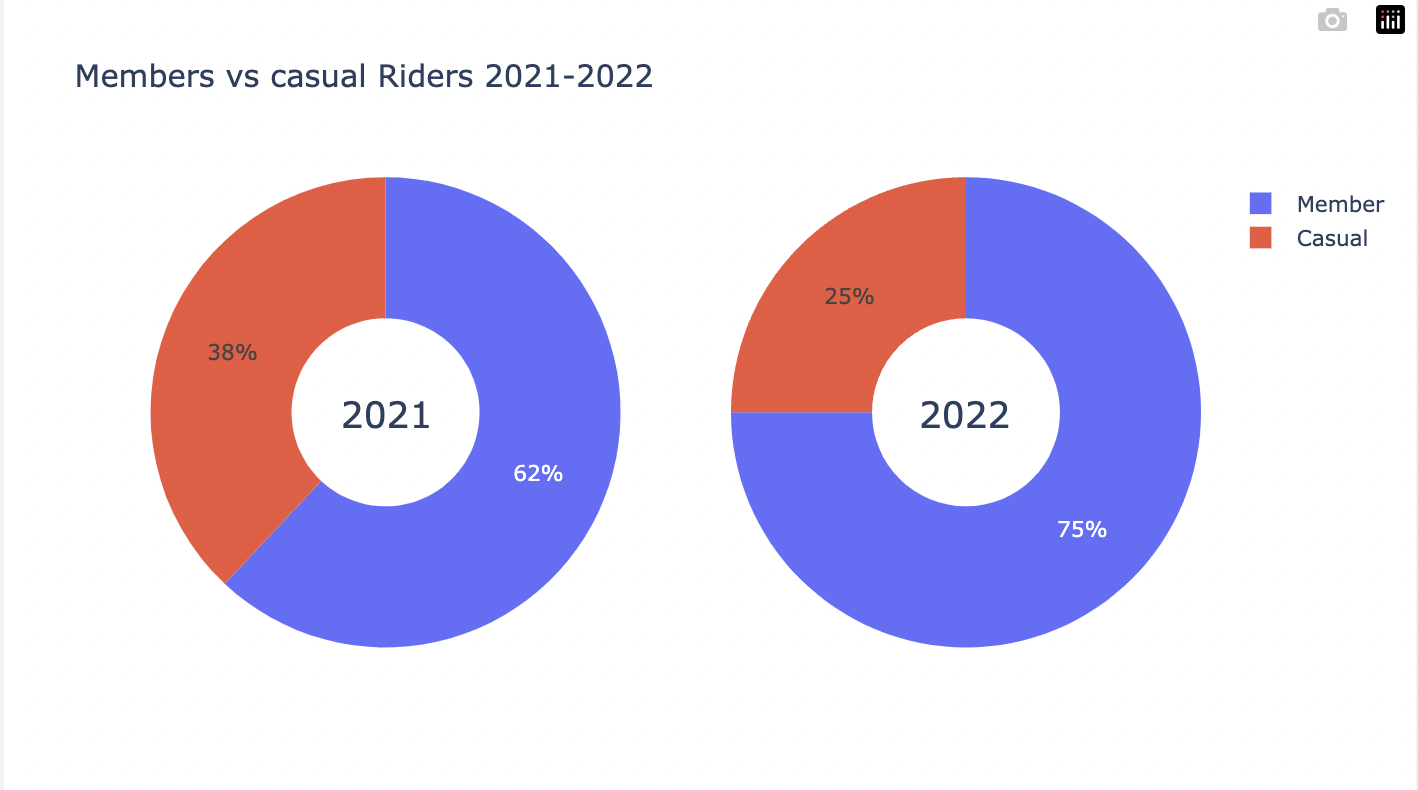
\includegraphics[width=3.3in, height=1.8in]{figs/subsc.png}\\
        \captionof{figure}{Subscription analysis of Citi bike in the years 2021 and 2022}}
\item \textbf{Gender Analysis and Subscription Analysis:} Finally, we will conduct a gender analysis and subscription analysis to better understand the demographics of Citi Bike users and their subscription patterns. This information can be used to ensure that the program is accessible and inclusive to all New Yorkers.
\end{enumerate}
\subsection{Models}
\subsubsection{LSTM}
    \item LSTMs can be used to model univariate time series forecasting problems.\cite{CNN} The LSTM model will learn a function that maps a sequence of past observations as input to an output observation. So initially we have trained an LSTM model for citi bike's ride forecasting. Here, we obtained the RMSE scores of each station in the range of 10 to 18.
\subsubsection{CNN-LSTM}
   \item In order to forecast the demand on per station basis, we trained our hybrid model on the number of rides started on a daily basis. \cite{CNN}The Hybrid CNN-LSTM models are popular for time series forecasting as they can capture both local and global temporal patterns and can perform timing analysis while extracting abstract features. The benefit of this model is that it can handle very long input sequences, which the CNN model may read as blocks or subsequences and then piece together by the LSTM model. The CNN model will interpret each sub-sequence and the LSTM will piece together the interpretations from the subsequences. Here the dataset for each station is split into 70/30 for training and validation. We trained around 750 stations to predict the future of rides for each station and the train time is around 10 hours. We used Rootmean squared error (RMSE) as the metric as it penalizes larger errors more heavily than smaller errors. After training the validation RMSE of each station is from the range 2 to 8. Here the figure 5 displays the Train loss va Validation loss for LSTM and CNN-LSTM models. It is evident that CNN-LSTM outbeats LSTM model as the train loss and validation loss of the CNN-LSTM model converge rapidly when compared to LSTM.
         
    \parbox{\linewidth}{
        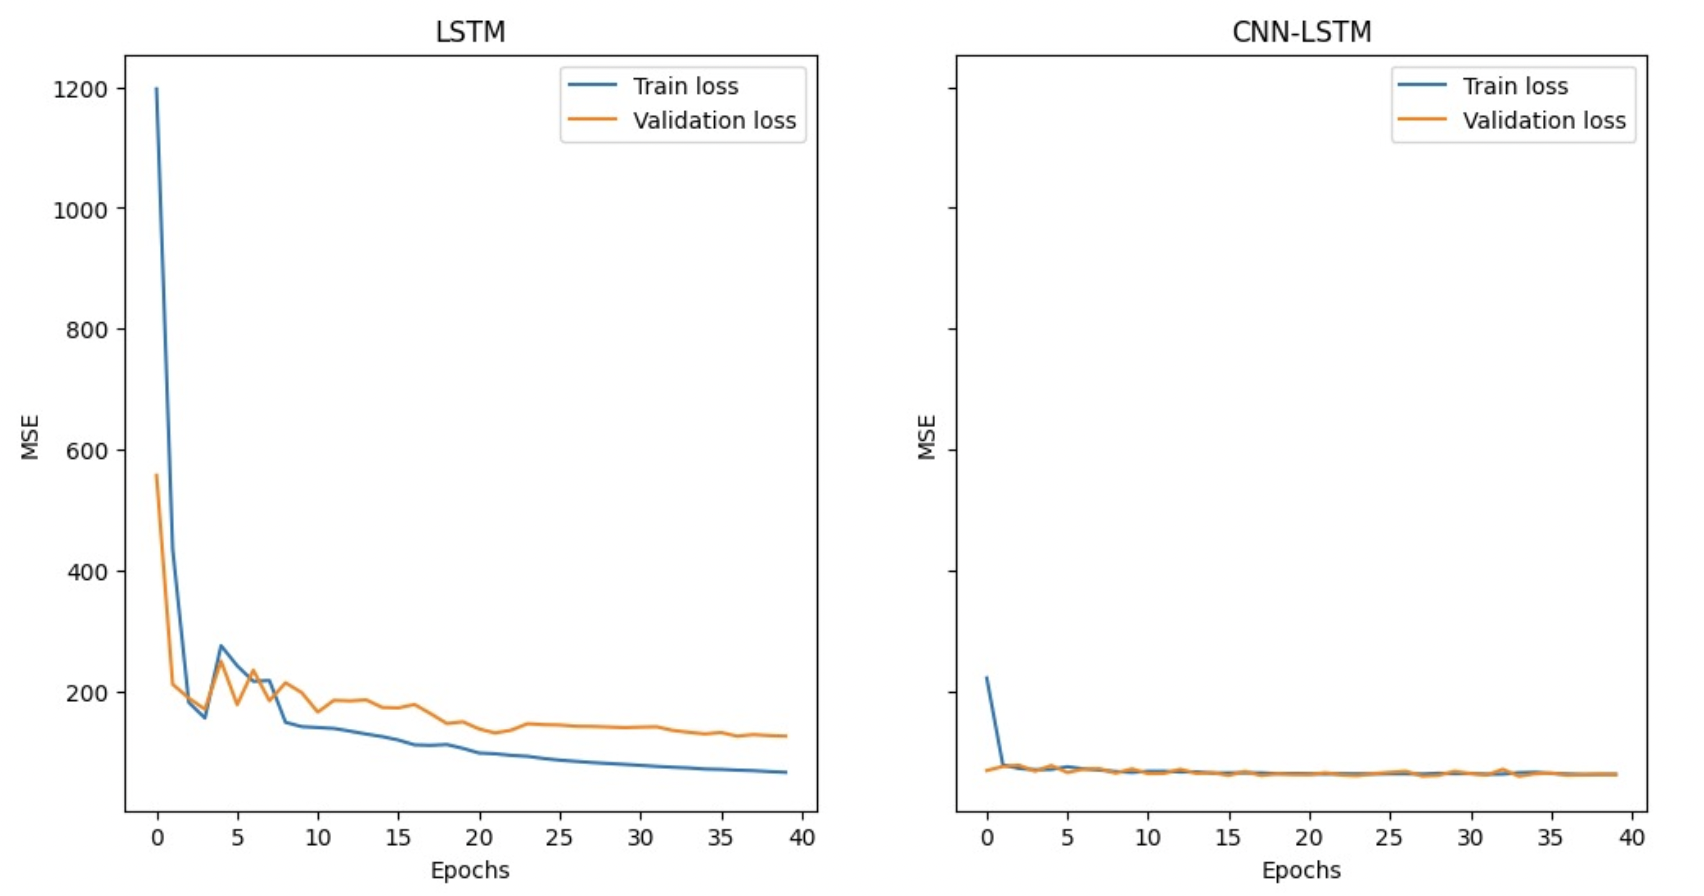
\includegraphics[width=3.4in, height=2in]{figs/model.png}\\
        \captionof{figure}{Train loss vs Val loss for LSTM and CNN-LSTM}
    }

\section{Results}
\subsection{Station Analysis and Distribution Variation \cite{11}:}
\begin{enumerate}
    \item Figure 2 shows the station analysis module. This module was inspired by the University of Southern California's Citibike visualization. We have improved the dataset by including every month's data and visualized them, including recent years (2018 - 2022), in this version, which is an extension of the previous version. We have included every month's data such that clicking on each station selecting the year and month shows the bar charts with the total no. of borrowed bikes and returned bikes per selected station. Each station displays hourly information on returned and borrowed bikes.
    
    \parbox{\linewidth}{
        \includegraphics[width=3.4in, height=2in]{figs/dist.png}\\
        \captionof{figure}{Distribution variation on stations} 
        }
    \item Distribution variation shows the statistics of the yearly data and the yearly variation of the bike rides with respect to stations. Figure 6 shows the variations of the years 2013 and 2018. The line plot is used for comparing the no. of rides in an hourly basis and the barchart below displays the updated stations and their counts respectively. Even here, we have updated the prior edition by including data from recent years (2018 - 2022).
\end{enumerate}
\parbox{\linewidth}{
        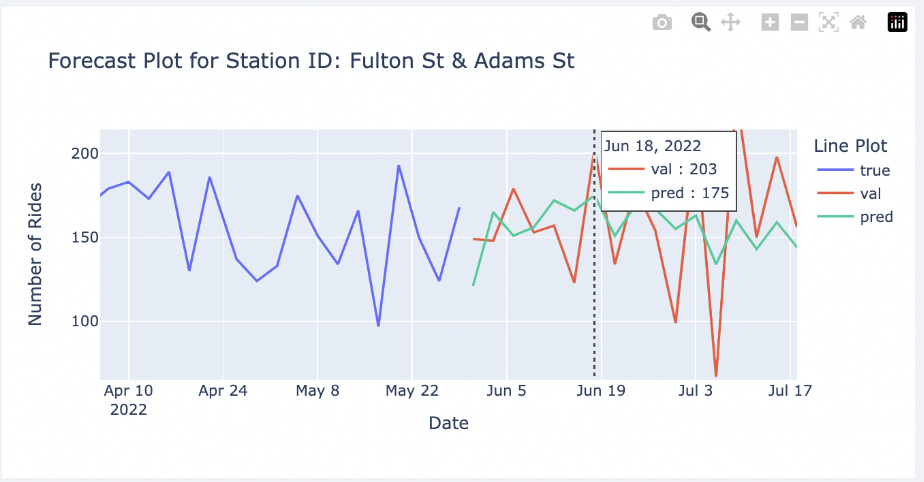
\includegraphics[width=3.4in, height=2in]{figs/forecast.png}\\
        \captionof{figure}{Forecasting plot of a station} 
        }
\subsection{Ride Forecasting:}
\begin{enumerate}
    \item Figure 1 shows the future rides forecasting of the specific station when selected on the map. Each forecasting plot shows shows the previous trend, true values and the predicted values of the future rides. 
    \item Blue line indicates the previous rides and the validation data is taken for 3 months of data. The X-axis diplays the no. of rides and the Y-axis shows the date of the specific rides. The predicted vs true values displays the validation plot of the model. 
    \item Figure 7 clearly displays the previous data and true vs predicted rides clearly. All these plots are trained with CNN-LSTM model which is the best model which could be used for this use case. All these plots are dynamic and interactive.
    \item These plots are spiky as they present daily data since the past 1 year. Smoothening these graphs could be included in the future scope of this paper.
\end{enumerate}
\parbox{\linewidth}{
        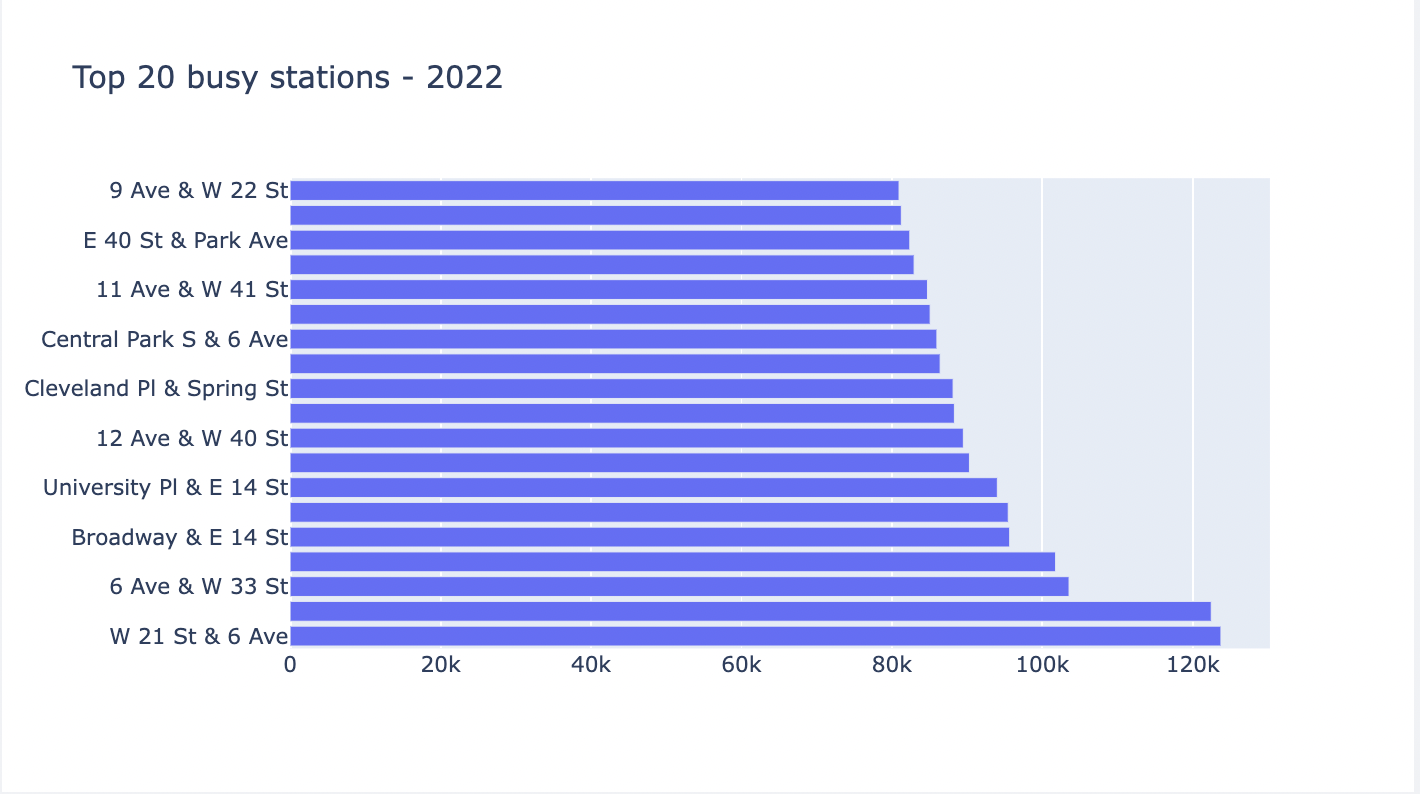
\includegraphics[width=3.4in, height=2in]{figs/busy.png}\\
        \captionof{figure}{Forecasting plot of a station} 
        }
\subsection{Top 20 busy stations analysis:}
\begin{enumerate}
\item This is a part of statistics page of our visualization dashboard. In this module we have analyzed top 20 stations where there is high demand for the bikes in the year 2022. This information is useful for the policy makers to increase the supply of citi bikes at these corresponding stations and increase the capacity of the station.
\item Figure 8 displays the horizontal bar chart where the X-axis displays the no. of rides and the Y-axis displays the Station names. From the analysis we have made, W 21st \& 6th avenue station has the highest number of rides with 123,745 rides and 6th avenue \& W 33 st has the second highest number of rides with 122,460 rides.
\end{enumerate}
\parbox{\linewidth}{
        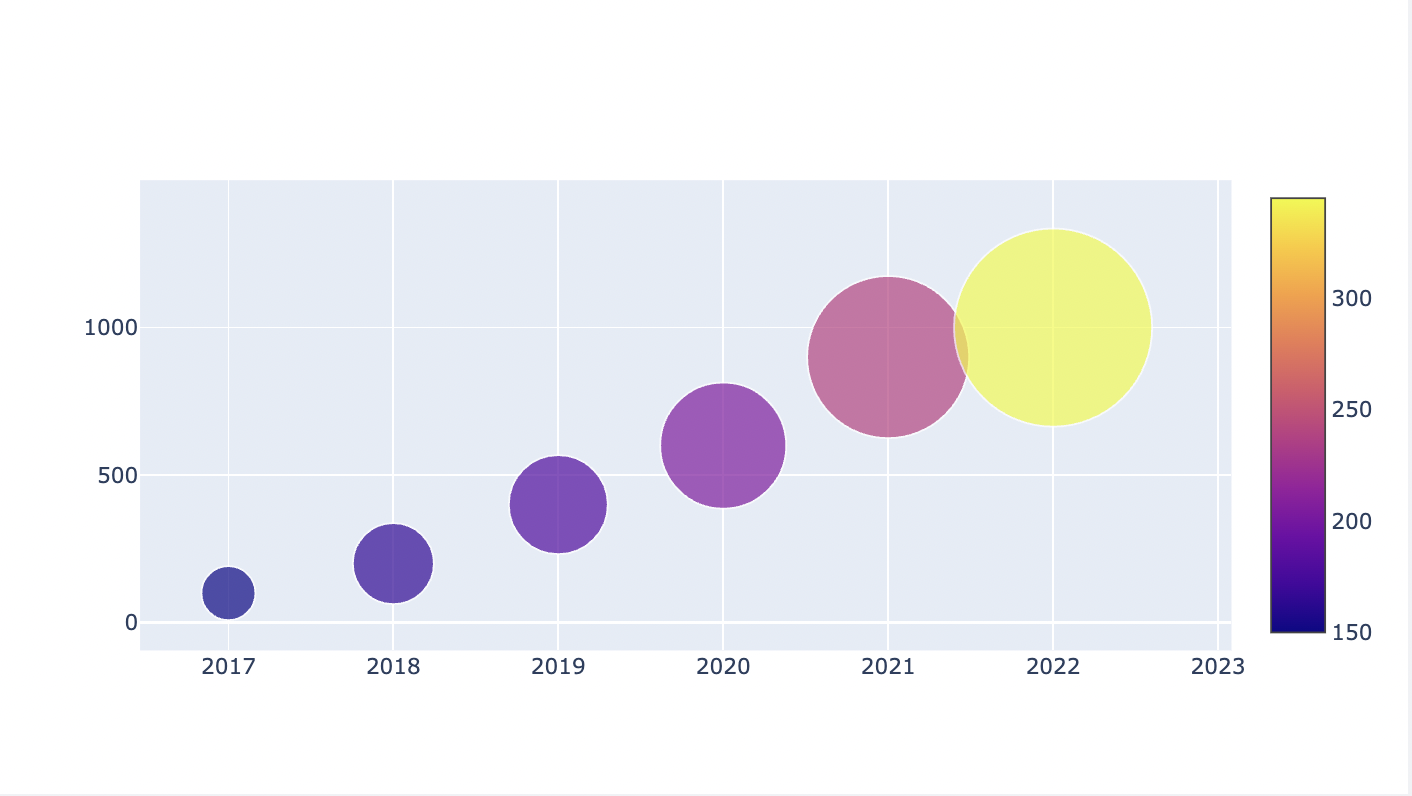
\includegraphics[width=3.4in, height=2in]{figs/demand.png}\\
        \captionof{figure}{Demand plot over the years} 
        }
\subsection{Ride Demand analysis:}
\begin{enumerate}
\item Here we have analysed the demand of the stations using no. of stations and the no. of rides over the years in a bubble scatter plot. This plot can help Citi bike decision-makers comprehend the demand for Citi bikes and analyze the increasing pattern over time.
\item Figure 9 here shows the demand plot for the citi bikes. X-axis indicates the total no. of rides in an year in thousands, Y-axis indicates the years and the area of the circle indicates the increasing no. of station count. 
\item This plot shows us that the demand for citibikes have been rapidly increasing over the years. As a result, they have to uphold their organization's standards of operation.
\end{enumerate}
\subsection{Gender Analysis and Subscription Analysis:}
\begin{enumerate}
    \item Figure 3 shows the gender analysis of citi bikes in the years 2021 and 2022. We have analysed this to show the gender effect on the no. of rides by pie chart. 
    \item This demonstrates that male riders outnumbered female riders by 30\% in 2022. The chart also shows that female cyclists have declined from 2021 to 2022. Hence there is a need for the organization to advertise themselves so that female riders will expand significantly.
    \item Figure 4 shows the subscription analysis of citi bikes in the years 2021 and 2022. We have analysed this to show the subscription effect on the no. of rides by donut chart.
    \item This shows that members oftenly use the bikes compared to the casual riders. Hence there is a need to campaign and market their application such that casual riders could easily access these bikes.
\end{enumerate}
\section{Future Scope and Conclusion}
There are several avenues for future improvements to the dashboard that can enhance its functionality and utility. One area for development is to further improve the accuracy of the forecasting model by integrating more sophisticated algorithms and techniques. Another area for exploration is to enhance the interactivity of the visualizations to facilitate user comprehension and exploration. Furthermore, streamlining the UI for the dashboard can make it even more user-friendly and accessible for a wider range of users. Finally, integrating the dashboard with the existing dashboard for multiple cities' bike-sharing ecosystems can provide users with a broader perspective on bike-sharing trends and patterns. In conclusion, we have successfully developed a dashboard for analyzing and reviewing New York City's bike-sharing dataset. The dashboard provides users with a wide range of visualizations and forecasting capabilities, making it a valuable tool for understanding bike-sharing trends and patterns. Our future goals include enhancing the accuracy of the forecasting model, improving the interactivity of the visualizations, streamlining the UI, and integrating the dashboard with other bike-sharing ecosystems. Overall, the dashboard has the potential to provide valuable insights into bike-sharing trends and facilitate better decision-making in the bike-sharing industry.

\section{References}

\begin{thebibliography}{9}
\bibitem{Parkes et al.}
Fishman, Elliot. (2015). Bikeshare: A Review of Recent Literature. Transport Reviews. 36. 10.1080/01441647.2015.1033036. 

\bibitem{lamport94}
Leslie Lamport (1994) \emph{\LaTeX: a document preparation system}, Addison
Wesley, Massachusetts, 2nd ed.

\bibitem{Faghih-imani}
Faghih-imani, A., Eluru, N., El-geneidy, A. M., Rabbat, M., & Haq, U. (2014). How land-use and urban form impact bicycle flows : evidence from the bicycle-sharing system ( BIXI ) in Montreal. Journal of Transport Geography, 41(August 2012), 306–314. https://doi.org/10.1016/j.jtrangeo.2014.01.013.

\bibitem{M}
Mátrai, T., & Tóth, J. (2016). Comparative Assessment of Public Bike Sharing Systems. Transportation Research Procedia, 14, 2344–2351. https://doi.org/10.1016/j.trpro.2016.05.26.

\bibitem{dataset}
NYC Citibike Dataset, \href{https://citibikenyc.com/system-data}{https://citibikenyc.com/system-data}

\bibitem{Meng}
Volume, M. E., Me, I., & Meng, O. (2011). Implementing bike-sharing systems, 164. https://doi.org/10.1680/muen.2011.164.2.8.

\bibitem{Zhao J}
Zhao J, Wang J, Deng W. Exploring bikesharing travel time and trip chain by gender and day of the week. Transportation Research Part C: Emerging Technologies. 2015; 58, Part B:251–64.  

\bibitem{Goodman A}
Goodman A, Cheshire J. Inequalities in the London bicycle sharing system revisited: impacts of extend- ing the scheme to poorer areas but then doubling prices. Journal of Transport Geography.  

\bibitem{Xiaonan Zhang}
Understanding the intention to use bike-sharing system: A case study in Xi’an, China.Xiaonan Zhang, Conceptualization, Methodology, Software, Writing – original draft, Writing – review & editing,Jianjun Wang, Supervision,# Xueqin Long, Data curation, Validation and Weijia Li, Investigation .

\bibitem{Yuan}
 Operating Characteristics of Dockless Bike-Sharing Systems near Metro Stations: Case Study in Nanjing City, China by Yuan Li,Zhenjun Zhu andXiucheng Guo .

\bibitem{August 2020}
Bikesharing, equity, and disadvantaged communities: A case study in Chicago August 2020 Transportation Research Part A Policy and Practice 140(3) DOI:10.1016/j.tra.2020.07.004.

\bibitem{11}
Citi Bike Information Visualization Jing Zhang, Tianyang Li, Ziwei Yuan, and Tong Lyu University of Southern California, Los Angeles CA 900007, USA  

\bibitem{YA}
Cleaner Production, 2014. [19] Y. Zheng, L. Capra, O. Wolfson, and H. Yang. Urban computing: concepts, methodologies, and applications. ACM Transaction on Intelligent Systems and Technology (ACM TIST), 2014.

\bibitem{X}
X. Wang, G. Lindsey, J. E. Schoner, and A. Harrison. Modeling bike share station activity: The eFects of nearby businesses and jobs on trips to and from stations. Transportation Research Record, 43(44):45, 2012.


\bibitem{CNN}
LSTM, CNN-LSTM for time series forecasting
\href{https://machinelearningmastery.com/how-to-get-started-with-deep-learning-for-time-series-forecasting-7-day-mini-course/}{https://machinelearningmastery.com/}




\end{thebibliography}

\end{document}

